\documentclass[11pt,a4paper]{ivoa}
\input tthdefs

\title{A componant based model for source data}

% see ivoatexDoc for what group names to use here
\ivoagroup{DM}


\author{François Bonnarel}
\author{Gilles Landais}
\author{Laurent Michel}

\editor{Laurent Michel}

% \previousversion[????URL????]{????Concise Document Label????}
\previousversion{This is the first public release}
       

\begin{document}
\begin{abstract}
???? Abstract ????
\end{abstract}


\section*{Acknowledgments}

???? Or remove the section header ????

\section*{Conformance-related definitions}

The words ``MUST'', ``SHALL'', ``SHOULD'', ``MAY'', ``RECOMMENDED'', and
``OPTIONAL'' (in upper or lower case) used in this document are to be
interpreted as described in IETF standard RFC2119 \citep{std:RFC2119}.

The \emph{Virtual Observatory (VO)} is a
general term for a collection of federated resources that can be used
to conduct astronomical research, education, and outreach.
The \href{http://www.ivoa.net}{International
Virtual Observatory Alliance (IVOA)} is a global
collaboration of separately funded projects to develop standards and
infrastructure that enable VO applications.


\section{Introduction}

???? Write something ????

\subsection{Role within the VO Architecture}

\begin{figure}
\centering

% As of ivoatex 1.2, the architecture diagram is generated by ivoatex in
% SVG; copy ivoatex/archdiag-full.xml to archdiag.xml and throw out
% all lines not relevant to your standard.
% Notes don't generally need this.  If you don't copy archdiag.xml,
% you must remove archdiag.svg from FIGURES in the Makefile.

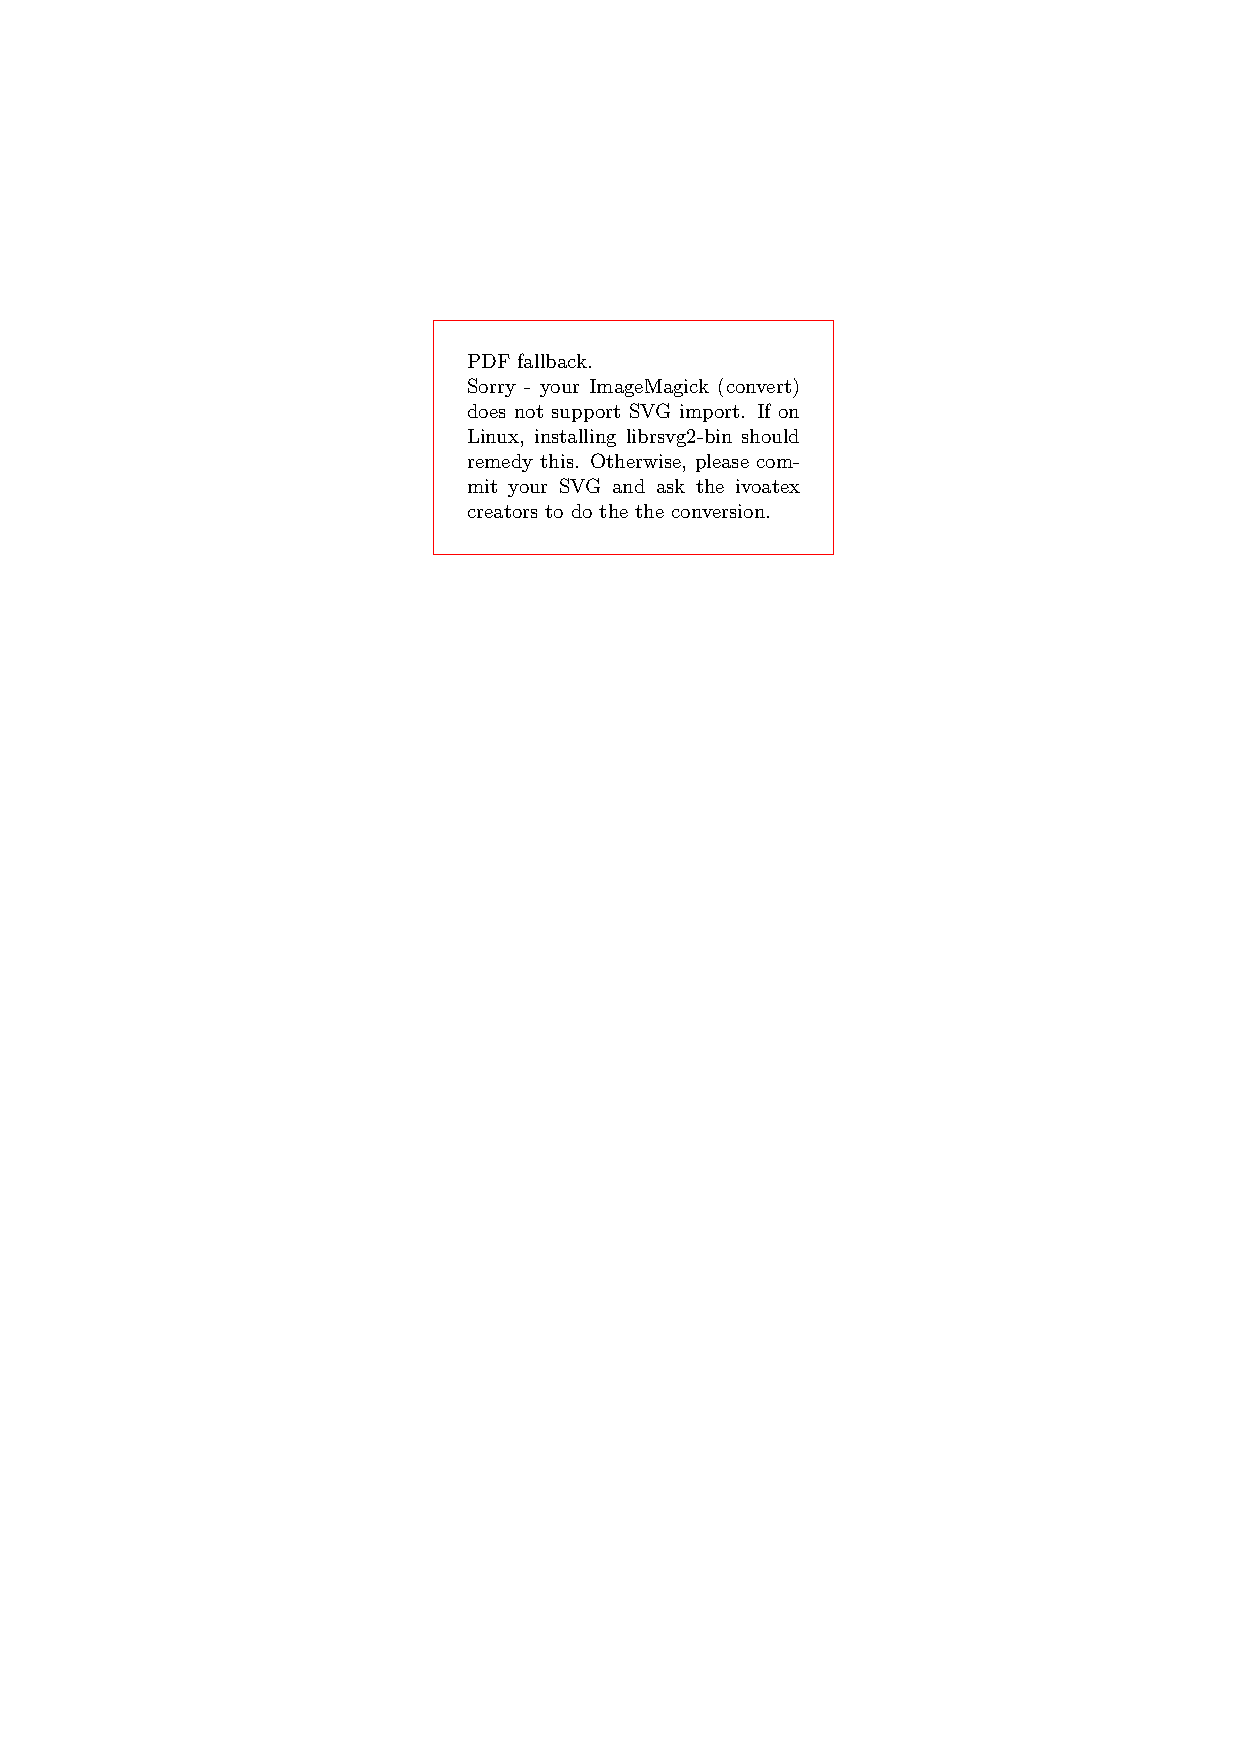
\includegraphics[width=0.9\textwidth]{role_diagram.pdf}
\caption{Architecture diagram for this document}
\label{fig:archdiag}
\end{figure}

Fig.~\ref{fig:archdiag} shows the role this document plays within the
IVOA architecture \citep{note:VOARCH}.



\section{Use Cases and  Requirements}



% -------------------------------------------
% Items to substitute into the ivoatex document template.
%
%\ivoagroup{Data Model Working Group}

%\title{Mango}


%\author{Laurent Michel}
    
%\author{François Bonnarel}
    
%\author{Gilles Landais}
    
%\author{Mireille Louys}
    
%\author{Marco Molinaro}
    
%\author{Jesue Salgado}
    
%\previousversion{0.0}
      
% -------------------------------------------

\pagebreak
\section{Model: mango }
  
  % INSERT FIGURE HERE
  %\begin{figure}[h]
  %\begin{center}
  %  \includegraphics[width=\textwidth]{????.png}
  %  \caption{???}\label{fig:????}
  %\end{center}
  %\end{figure}

  Data model based oon components and data association for source data

  \subsection{AssociatedData (Abstract)}
  \label{sect:AssociatedData}
    Abstract reference to a particular dataset associated to the Source. This class is used to specify the type of the dataset as well as its role.

    \subsubsection{AssociatedData.semantic}
      \textbf{vodml-id: AssociatedData.semantic} \newline
      \textbf{type: \hyperref[sect:stcextend.RDFWord]{mango:stcextend.RDFWord}} \newline
      \textbf{multiplicity: 1} \newline 
      Reference to a semantic concept giving the nature of the associated data. As long as the vocabulary is not set, the possible values of this attribute are given by the LinkSemantic enumeration.

    \subsubsection{AssociatedData.dataType}
      \textbf{vodml-id: AssociatedData.dataType} \newline
      \textbf{type: \hyperref[sect:ivoa]{ivoa:string}} \newline
      \textbf{multiplicity: 1} \newline 
      Type of the associated data (not defined yet)

    \subsubsection{AssociatedData.description}
      \textbf{vodml-id: AssociatedData.description} \newline
      \textbf{type: \hyperref[sect:ivoa]{ivoa:string}} \newline
      \textbf{multiplicity: 1} \newline 
      Free text description of the associated data

  \subsection{HardnessRatioSys}
  \label{sect:HardnessRatioSys}
    TODO : Missing description : please, update your UML model asap.

    \noindent \textbf{subset} \newline
    \indent   \textbf{role: coords:PhysicalCoordSys.frame} \newline
    \indent   \textbf{type: mango:HRFrame} \newline


  \subsection{MangoInstance}
  \label{sect:MangoInstance}
    Reference to another CAB-MSD instance that is part of the associated data.

    \subsubsection{MangoInstance.mangoInstance}
      \textbf{vodml-id: MangoInstance.mangoInstance} \newline
      \textbf{type: \hyperref[sect:Source]{mango:Source}} \newline
      \textbf{multiplicity: 1} \newline 
      Composition link pointing on one cab\_msd instance associated with the source.

  \subsection{ModelInstance}
  \label{sect:ModelInstance}
    Placeholder for the mapping of the model instance

  \subsection{Parameter}
  \label{sect:Parameter}
    Reference to a particular measure of the Source. This class is used to specify the type of the measure as well as its role.

    \noindent \textbf{constraint} \newline
    \indent    \textbf{detail: Parameter.One association at the time
 }\newline


    \subsubsection{Parameter.semantic}
      \textbf{vodml-id: Parameter.semantic} \newline
      \textbf{type: \hyperref[sect:stcextend.RDFWord]{mango:stcextend.RDFWord}} \newline
      \textbf{multiplicity: 1} \newline 
      Reference to a semantic concept giving the nature of the parameter As long as the vocabulary is not set, the possible values of this attribute are given by the ParamSemantic enumeration.

    \subsubsection{Parameter.ucd}
      \textbf{vodml-id: Parameter.ucd} \newline
      \textbf{type: \hyperref[sect:ivoa]{ivoa:string}} \newline
      \textbf{multiplicity: 1} \newline 
      UCD1+ giving the type of the physical measure

    \subsubsection{Parameter.description}
      \textbf{vodml-id: Parameter.description} \newline
      \textbf{type: \hyperref[sect:ivoa]{ivoa:string}} \newline
      \textbf{multiplicity: 1} \newline 
      Free text description of the measure

    \subsubsection{Parameter.measure}
      \textbf{vodml-id: Parameter.measure} \newline
      \textbf{type: meas:Measure} \newline
      \textbf{multiplicity: 1} \newline 
      Composition link pointing to the meas:Measure instance

    \subsubsection{Parameter.associatedParameters}
      \textbf{vodml-id: Parameter.associatedParameters} \newline
      \textbf{type: \hyperref[sect:Parameter]{mango:Parameter}} \newline
      \textbf{multiplicity: 0..*} \newline 
      TODO : Missing description : please, update your UML model asap.

  \subsection{PhotometryCoordSys}
  \label{sect:PhotometryCoordSys}
    TODO : Missing description : please, update your UML model asap.

    \noindent \textbf{subset} \newline
    \indent   \textbf{role: coords:PhysicalCoordSys.frame} \newline
    \indent   \textbf{type: mango:PhotFilter} \newline


  \subsection{Source}
  \label{sect:Source}
    Root class of the model. CAB\_MSF instance are meant ot be Source instances. A source ha an identifier and to sets of hooks: one for the parameters and one for the associated data.

    \subsubsection{Source.identifier}
      \textbf{vodml-id: Source.identifier} \newline
      \textbf{type: \hyperref[sect:ivoa]{ivoa:string}} \newline
      \textbf{multiplicity: 1} \newline 
      Unique identifier for a Source. The uniqness of that identifier is not managed by the model. The format is free.

    \subsubsection{Source.associatedData}
      \textbf{vodml-id: Source.associatedData} \newline
      \textbf{type: \hyperref[sect:AssociatedData]{mango:AssociatedData}} \newline
      \textbf{multiplicity: 0..*} \newline 
      Composition link pointing on all data associated with the source.

    \subsubsection{Source.parameters}
      \textbf{vodml-id: Source.parameters} \newline
      \textbf{type: \hyperref[sect:Parameter]{mango:Parameter}} \newline
      \textbf{multiplicity: 0..*} \newline 
      Composition link pointing on all parameters attached to the source.

  \subsection{Temperature}
  \label{sect:Temperature}
    TODO : Missing description : please, update your UML model asap.

    \subsubsection{Temperature.coord}
      \textbf{vodml-id: Temperature.coord} \newline
      \textbf{type: \hyperref[sect:ivoa]{ivoa:string}} \newline
      \textbf{multiplicity: 1} \newline 
      TODO : Missing description : please, update your UML model asap.

  \subsection{VOModelInstance}
  \label{sect:VOModelInstance}
    Reference to a VO model instance that is part of the associated data.

    \subsubsection{VOModelInstance.ivoid}
      \textbf{vodml-id: VOModelInstance.ivoid} \newline
      \textbf{type: \hyperref[sect:ivoa]{ivoa:string}} \newline
      \textbf{multiplicity: 1} \newline 
      VO-DML id of the referenced model

    \subsubsection{VOModelInstance.modelUrl}
      \textbf{vodml-id: VOModelInstance.modelUrl} \newline
      \textbf{type: \hyperref[sect:ivoa]{ivoa:anyURI}} \newline
      \textbf{multiplicity: 1} \newline 
      URL on the VO-DML model

    \subsubsection{VOModelInstance.modelName}
      \textbf{vodml-id: VOModelInstance.modelName} \newline
      \textbf{type: \hyperref[sect:ivoa]{ivoa:string}} \newline
      \textbf{multiplicity: 1} \newline 
      Name of the referenced model

    \subsubsection{VOModelInstance.modelDoc}
      \textbf{vodml-id: VOModelInstance.modelDoc} \newline
      \textbf{type: \hyperref[sect:ivoa]{ivoa:anyURI}} \newline
      \textbf{multiplicity: 1} \newline 
      Documentation URL of the model

    \subsubsection{VOModelInstance.modelInstance}
      \textbf{vodml-id: VOModelInstance.modelInstance} \newline
      \textbf{type: \hyperref[sect:ModelInstance]{mango:ModelInstance}} \newline
      \textbf{multiplicity: 1} \newline 
      Composition link pointing on one VO instance instance associated with the source.

  \subsection{VOService}
  \label{sect:VOService}
    Class for associated data referenced by an URL that is a VO service

    \subsubsection{VOService.ivoid}
      \textbf{vodml-id: VOService.ivoid} \newline
      \textbf{type: \hyperref[sect:ivoa]{ivoa:string}} \newline
      \textbf{multiplicity: 1} \newline 
      IVOA id attached to the URI

  \subsection{WebEndpoint}
  \label{sect:WebEndpoint}
    Class for associated data referenced by an URL

    \subsubsection{WebEndpoint.ContentType}
      \textbf{vodml-id: WebEndpoint.ContentType} \newline
      \textbf{type: \hyperref[sect:ivoa]{ivoa:string}} \newline
      \textbf{multiplicity: 1} \newline 
      Mime type of the URL

    \subsubsection{WebEndpoint.url}
      \textbf{vodml-id: WebEndpoint.url} \newline
      \textbf{type: \hyperref[sect:ivoa]{ivoa:anyURI}} \newline
      \textbf{multiplicity: 1} \newline 
      Web endpoint

  \subsection{LinkSemantic}
  \label{sect:LinkSemantic}

  Literal enumeration of the possible values for the associated data semantic. This stands for an example before we have defined a vocabulary.

  \noindent \underline{Enumeration Literals}
  \vspace{-\parsep}
  \small
  \begin{itemize}
  
    \item[\textbf{VOService}]: \textbf{vodml-id:} LinkSemantic.VOService \newline
          \textbf{description:} Data returned by a VO service
    \item[\textbf{VOInstance}]: \textbf{vodml-id:} LinkSemantic.VOInstance \newline
          \textbf{description:} Data Serialized in a VO model
    \item[\textbf{Preview}]: \textbf{vodml-id:} LinkSemantic.Preview \newline
          \textbf{description:} data preview
    \item[\textbf{DownloadLink}]: \textbf{vodml-id:} LinkSemantic.DownloadLink \newline
          \textbf{description:} Data download link
    \item[\textbf{Detection}]: \textbf{vodml-id:} LinkSemantic.Detection \newline
          \textbf{description:} Particular detection
    \item[\textbf{Compagnon}]: \textbf{vodml-id:} LinkSemantic.Compagnon \newline
          \textbf{description:} Compagnon source
    \item[\textbf{Counterpart}]: \textbf{vodml-id:} LinkSemantic.Counterpart \newline
          \textbf{description:} Counter part source
  \end{itemize}
  \normalsize


  \subsection{ParamSemantic}
  \label{sect:ParamSemantic}

  Literal enumeration of the possible values for the parameter semantic. This stands for an example before we have defined a vocabulary.

  \noindent \underline{Enumeration Literals}
  \vspace{-\parsep}
  \small
  \begin{itemize}
  
    \item[\textbf{Main}]: \textbf{vodml-id:} ParamSemantic.Main \newline
          \textbf{description:} Main measurment
    \item[\textbf{Computed}]: \textbf{vodml-id:} ParamSemantic.Computed \newline
          \textbf{description:} Computed measurement
    \item[\textbf{Native}]: \textbf{vodml-id:} ParamSemantic.Native \newline
          \textbf{description:} Mative measurement
    \item[\textbf{Raw}]: \textbf{vodml-id:} ParamSemantic.Raw \newline
          \textbf{description:} raw measure
    \item[\textbf{Corrected}]: \textbf{vodml-id:} ParamSemantic.Corrected \newline
          \textbf{description:} Corrected measure
  \end{itemize}
  \normalsize


\pagebreak
\section{Package: stcextend }

  % INSERT FIGURE HERE
  %\begin{figure}[h]
  %\begin{center}
  %  \includegraphics[width=\textwidth]{????.png}
  %  \caption{???}\label{fig:????}
  %\end{center}
  %\end{figure}

  This package contains all object and type classes that has been extended from the Measure and Coordinates models. This extension mechanism is used to add new types of measures while staying whithin the Mes/Coords pattern.

  \subsection{Flag}
  \label{sect:stcextend.Flag}
    Measure to be used for status parameters

    \subsubsection{Flag.coord}
      \textbf{vodml-id: stcextend.Flag.coord} \newline
      \textbf{type: \hyperref[sect:stcextend.FlagCoord]{mango:stcextend.FlagCoord}} \newline
      \textbf{multiplicity: 1} \newline 
      Coordinate holding the statsu value

  \subsection{FlagCoord}
  \label{sect:stcextend.FlagCoord}
    Coordinate of a status Measure

    \noindent \textbf{subset} \newline
    \indent   \textbf{role: coords:Coordinate.coordSys} \newline
    \indent   \textbf{type: FlagSys} \newline


    \subsubsection{FlagCoord.status}
      \textbf{vodml-id: stcextend.FlagCoord.status} \newline
      \textbf{type: \hyperref[sect:ivoa]{ivoa:integer}} \newline
      \textbf{multiplicity: 1} \newline 
      Value of the status

  \subsection{FlagState}
  \label{sect:stcextend.FlagState}
    Possible value of a status

    \subsubsection{FlagState.value}
      \textbf{vodml-id: stcextend.FlagState.value} \newline
      \textbf{type: \hyperref[sect:ivoa]{ivoa:integer}} \newline
      \textbf{multiplicity: 1} \newline 
      Status value

    \subsubsection{FlagState.label}
      \textbf{vodml-id: stcextend.FlagState.label} \newline
      \textbf{type: \hyperref[sect:ivoa]{ivoa:string}} \newline
      \textbf{multiplicity: 1} \newline 
      Label attached to that status value

  \subsection{FlagSys}
  \label{sect:stcextend.FlagSys}
    Coordinate system to be used for statur measures.

    \subsubsection{FlagSys.statusLabel}
      \textbf{vodml-id: stcextend.FlagSys.statusLabel} \newline
      \textbf{type: \hyperref[sect:stcextend.FlagState]{mango:stcextend.FlagState}} \newline
      \textbf{multiplicity: 0..*} \newline 
      Composition loink to all possible status values for this system

  \subsection{HRFrame}
  \label{sect:stcextend.HRFrame}
    Hardness ratio frame. Defined by 2 energy bands Eheigh ELow. HR = (Eheigh - Elow)/(Eheigh + Elow) Energy bands are deemed to special photometric filters

    \subsubsection{HRFrame.low}
      \textbf{vodml-id: stcextend.HRFrame.low} \newline
      \textbf{type: \hyperref[sect:stcextend.PhotFilter]{mango:stcextend.PhotFilter}} \newline
      \textbf{multiplicity: 1} \newline 
      Low energy band

    \subsubsection{HRFrame.high}
      \textbf{vodml-id: stcextend.HRFrame.high} \newline
      \textbf{type: \hyperref[sect:stcextend.PhotFilter]{mango:stcextend.PhotFilter}} \newline
      \textbf{multiplicity: 1} \newline 
      Heigh energy band

  \subsection{HardnessRatio}
  \label{sect:stcextend.HardnessRatio}
    TODO : Missing description : please, update your UML model asap.

    \subsubsection{HardnessRatio.coord}
      \textbf{vodml-id: stcextend.HardnessRatio.coord} \newline
      \textbf{type: \hyperref[sect:stcextend.HardnessRatioCoord]{mango:stcextend.HardnessRatioCoord}} \newline
      \textbf{multiplicity: 1} \newline 
      TODO : Missing description : please, update your UML model asap.

  \subsection{HardnessRatioCoord}
  \label{sect:stcextend.HardnessRatioCoord}
    TODO : Missing description : please, update your UML model asap.

    \noindent \textbf{subset} \newline
    \indent   \textbf{role: coords:Coordinate.coordSys} \newline
    \indent   \textbf{type: mango:HardnessRatioSys} \newline


    \subsubsection{HardnessRatioCoord.hardnessRatio}
      \textbf{vodml-id: stcextend.HardnessRatioCoord.hardnessRatio} \newline
      \textbf{type: \hyperref[sect:ivoa]{ivoa:real}} \newline
      \textbf{multiplicity: 1} \newline 
      TODO : Missing description : please, update your UML model asap.

  \subsection{LonLatCoordSys}
  \label{sect:stcextend.LonLatCoordSys}
    TODO : Missing description : please, update your UML model asap.

    \noindent \textbf{subset} \newline
    \indent   \textbf{role: coords:PhysicalCoordSys.frame} \newline
    \indent   \textbf{type: coords:SpaceFrame} \newline


    \noindent \textbf{constraint} \newline
    \indent    \textbf{detail: LonLatCoordSys.coordSpace[0] }\newline


  \subsection{LonLatPoint}
  \label{sect:stcextend.LonLatPoint}
    Coordinate of a point on the sky sphere expressed in spherical coordinates.

    \noindent \textbf{subset} \newline
    \indent   \textbf{role: coords:Coordinate.coordSys} \newline
    \indent   \textbf{type: mango:LonLatCoordSys} \newline


    \subsubsection{LonLatPoint.longitude}
      \textbf{vodml-id: stcextend.LonLatPoint.longitude} \newline
      \textbf{type: \hyperref[sect:ivoa]{ivoa:real}} \newline
      \textbf{multiplicity: 1} \newline 
      longitude of the point

    \subsubsection{LonLatPoint.latitude}
      \textbf{vodml-id: stcextend.LonLatPoint.latitude} \newline
      \textbf{type: \hyperref[sect:ivoa]{ivoa:real}} \newline
      \textbf{multiplicity: 1} \newline 
      Latitude of the point

  \subsection{LonLatSkyPosition}
  \label{sect:stcextend.LonLatSkyPosition}
    Measure to used for sky points expressed with a spherical coordinate system

    \subsubsection{LonLatSkyPosition.coord}
      \textbf{vodml-id: stcextend.LonLatSkyPosition.coord} \newline
      \textbf{type: \hyperref[sect:stcextend.LonLatPoint]{mango:stcextend.LonLatPoint}} \newline
      \textbf{multiplicity: 1} \newline 
      Coordinate of spherical sky position

  \subsection{ObjectType}
  \label{sect:stcextend.ObjectType}
    TODO : Missing description : please, update your UML model asap.

    \subsubsection{ObjectType.coord}
      \textbf{vodml-id: stcextend.ObjectType.coord} \newline
      \textbf{type: \hyperref[sect:stcextend.OrbitCoord]{mango:stcextend.OrbitCoord}} \newline
      \textbf{multiplicity: 1} \newline 
      TODO : Missing description : please, update your UML model asap.

  \subsection{ObjectTypeCoord}
  \label{sect:stcextend.ObjectTypeCoord}
    TODO : Missing description : please, update your UML model asap.

    \noindent \textbf{subset} \newline
    \indent   \textbf{role: coords:Coordinate.coordSys} \newline
    \indent   \textbf{type: ObjectTypeSys} \newline


    \subsubsection{ObjectTypeCoord.objectType}
      \textbf{vodml-id: stcextend.ObjectTypeCoord.objectType} \newline
      \textbf{type: \hyperref[sect:ivoa]{ivoa:string}} \newline
      \textbf{multiplicity: 1} \newline 
      TODO : Missing description : please, update your UML model asap.

  \subsection{ObjectTypeSys}
  \label{sect:stcextend.ObjectTypeSys}
    TODO : Missing description : please, update your UML model asap.

  \subsection{Orbit}
  \label{sect:stcextend.Orbit}
    TODO : Missing description : please, update your UML model asap.

    \subsubsection{Orbit.coord}
      \textbf{vodml-id: stcextend.Orbit.coord} \newline
      \textbf{type: \hyperref[sect:stcextend.OrbitCoord]{mango:stcextend.OrbitCoord}} \newline
      \textbf{multiplicity: 1} \newline 
      TODO : Missing description : please, update your UML model asap.

  \subsection{OrbitCoord}
  \label{sect:stcextend.OrbitCoord}
    TODO : Missing description : please, update your UML model asap.

    \noindent \textbf{subset} \newline
    \indent   \textbf{role: coords:Coordinate.coordSys} \newline
    \indent   \textbf{type: coords:SpaceSys} \newline


  \subsection{PhotFilter}
  \label{sect:stcextend.PhotFilter}
    Photometric filter description, compliant with photDM

    \subsubsection{PhotFilter.name}
      \textbf{vodml-id: stcextend.PhotFilter.name} \newline
      \textbf{type: \hyperref[sect:ivoa]{ivoa:string}} \newline
      \textbf{multiplicity: 1} \newline 
      Filter name

    \subsubsection{PhotFilter.zeroPointFlux}
      \textbf{vodml-id: stcextend.PhotFilter.zeroPointFlux} \newline
      \textbf{type: \hyperref[sect:ivoa]{ivoa:real}} \newline
      \textbf{multiplicity: 1} \newline 
      Zero point flux of the filter

    \subsubsection{PhotFilter.magnitudeSystem}
      \textbf{vodml-id: stcextend.PhotFilter.magnitudeSystem} \newline
      \textbf{type: \hyperref[sect:ivoa]{ivoa:string}} \newline
      \textbf{multiplicity: 1} \newline 
      Magnitude system used by the filter

    \subsubsection{PhotFilter.effectiveWavelength}
      \textbf{vodml-id: stcextend.PhotFilter.effectiveWavelength} \newline
      \textbf{type: \hyperref[sect:ivoa]{ivoa:real}} \newline
      \textbf{multiplicity: 1} \newline 
      Effective wavelength of the filter

    \subsubsection{PhotFilter.unit}
      \textbf{vodml-id: stcextend.PhotFilter.unit} \newline
      \textbf{type: \hyperref[sect:ivoa]{ivoa:Unit}} \newline
      \textbf{multiplicity: 1} \newline 
      Wavelength unit used for that filter

    \subsubsection{PhotFilter.bandWidth}
      \textbf{vodml-id: stcextend.PhotFilter.bandWidth} \newline
      \textbf{type: \hyperref[sect:ivoa]{ivoa:real}} \newline
      \textbf{multiplicity: 1} \newline 
      Band width of the filter

  \subsection{Photometry}
  \label{sect:stcextend.Photometry}
    TODO : Missing description : please, update your UML model asap.

    \subsubsection{Photometry.coord}
      \textbf{vodml-id: stcextend.Photometry.coord} \newline
      \textbf{type: \hyperref[sect:stcextend.PhotometryCoord]{mango:stcextend.PhotometryCoord}} \newline
      \textbf{multiplicity: 1} \newline 
      TODO : Missing description : please, update your UML model asap.

  \subsection{PhotometryCoord}
  \label{sect:stcextend.PhotometryCoord}
    TODO : Missing description : please, update your UML model asap.

    \noindent \textbf{subset} \newline
    \indent   \textbf{role: coords:Coordinate.coordSys} \newline
    \indent   \textbf{type: PhotometryCoordSys} \newline


    \subsubsection{PhotometryCoord.luminosity}
      \textbf{vodml-id: stcextend.PhotometryCoord.luminosity} \newline
      \textbf{type: \hyperref[sect:ivoa]{ivoa:real}} \newline
      \textbf{multiplicity: 1} \newline 
      TODO : Missing description : please, update your UML model asap.

  \subsection{RDFWord}
  \label{sect:stcextend.RDFWord}
    Datatype for vocabulary word. Provides a pointer to the word description and a label.

    \subsubsection{RDFWord.rdf\_uri}
      \textbf{vodml-id: stcextend.RDFWord.rdf\_uri} \newline
      \textbf{type: \hyperref[sect:ivoa]{ivoa:string}} \newline
      \textbf{multiplicity: 1} \newline 
      URI extarcted from the DRF document and refering ot the word

    \subsubsection{RDFWord.label}
      \textbf{vodml-id: stcextend.RDFWord.label} \newline
      \textbf{type: \hyperref[sect:ivoa]{ivoa:string}} \newline
      \textbf{multiplicity: 1} \newline 
      RDF label. Matched the URL fragment for IVOA vocabularies

  \subsection{Redshift}
  \label{sect:stcextend.Redshift}
    TODO : Missing description : please, update your UML model asap.

    \subsubsection{Redshift.coord}
      \textbf{vodml-id: stcextend.Redshift.coord} \newline
      \textbf{type: \hyperref[sect:stcextend.RedshiftCoord]{mango:stcextend.RedshiftCoord}} \newline
      \textbf{multiplicity: 1} \newline 
      TODO : Missing description : please, update your UML model asap.

  \subsection{RedshiftCoord}
  \label{sect:stcextend.RedshiftCoord}
    TODO : Missing description : please, update your UML model asap.

    \noindent \textbf{subset} \newline
    \indent   \textbf{role: coords:Coordinate.coordSys} \newline
    \indent   \textbf{type: RedshiftSys} \newline


    \subsubsection{RedshiftCoord.redshift}
      \textbf{vodml-id: stcextend.RedshiftCoord.redshift} \newline
      \textbf{type: \hyperref[sect:ivoa]{ivoa:real}} \newline
      \textbf{multiplicity: 1} \newline 
      TODO : Missing description : please, update your UML model asap.

  \subsection{RedshiftSys}
  \label{sect:stcextend.RedshiftSys}
    TODO : Missing description : please, update your UML model asap.

  \subsection{Shape}
  \label{sect:stcextend.Shape}
    Measure giving the shape of a source

    \subsubsection{Shape.coord}
      \textbf{vodml-id: stcextend.Shape.coord} \newline
      \textbf{type: \hyperref[sect:stcextend.ShapeCoord]{mango:stcextend.ShapeCoord}} \newline
      \textbf{multiplicity: 1} \newline 
      String serialization of the source shape

  \subsection{ShapeCoord}
  \label{sect:stcextend.ShapeCoord}
    TODO : Missing description : please, update your UML model asap.

    \noindent \textbf{subset} \newline
    \indent   \textbf{role: coords:Coordinate.coordSys} \newline
    \indent   \textbf{type: ShapeSys} \newline


    \subsubsection{ShapeCoord.shape}
      \textbf{vodml-id: stcextend.ShapeCoord.shape} \newline
      \textbf{type: \hyperref[sect:ivoa]{ivoa:string}} \newline
      \textbf{multiplicity: 1} \newline 
      TODO : Missing description : please, update your UML model asap.

  \subsection{ShapeSys}
  \label{sect:stcextend.ShapeSys}
    Coordinate systen to be used for shape measure

    \subsubsection{ShapeSys.shapeFrame}
      \textbf{vodml-id: stcextend.ShapeSys.shapeFrame} \newline
      \textbf{type: \hyperref[sect:stcextend.ShapeFrame]{mango:stcextend.ShapeFrame}} \newline
      \textbf{multiplicity: 1} \newline 
      Frame of the shape measure. Gives a enumeration of the supported serializations.

  \subsection{ShapeFrame}
  \label{sect:stcextend.ShapeFrame}

  Enumeration of the possible options to encode a shape in a string.

  \noindent \underline{Enumeration Literals}
  \vspace{-\parsep}
  \small
  \begin{itemize}
  
    \item[\textbf{MOC}]: \textbf{vodml-id:} stcextend.ShapeFrame.MOC \newline
          \textbf{description:} MOC serialization
    \item[\textbf{STCs}]: \textbf{vodml-id:} stcextend.ShapeFrame.STCs \newline
          \textbf{description:} STCs serialization
  \end{itemize}
  \normalsize



\section{Model}
\subsection{Overview}
\begin{figure}
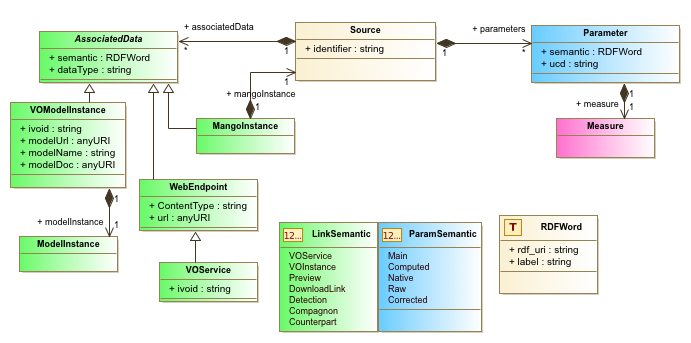
\includegraphics[width=0.9\textwidth]{../model/overview_diagram.png}
\caption{Architecture diagram for this document}
\label{fig:archdiag}
\end{figure}

\subsection{STC Extensions}

\begin{figure}
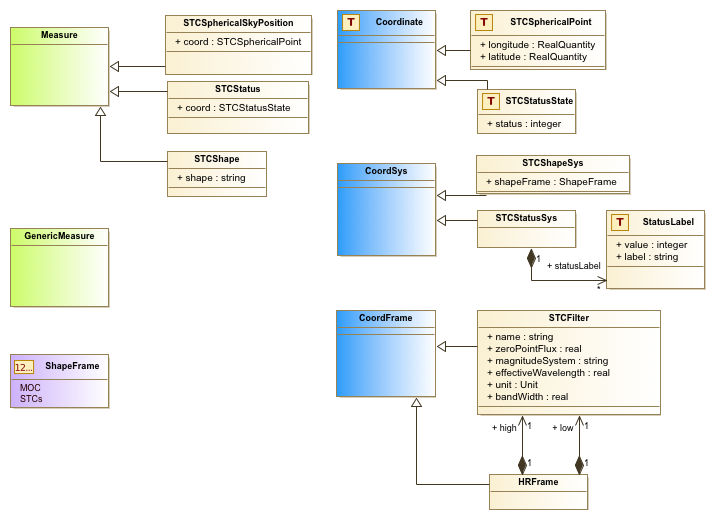
\includegraphics[width=0.9\textwidth]{../model/stc_ext_diagram.png}
\caption{Architecture diagram for this document}
\label{fig:archdiag}
\end{figure}

\appendix
\section{Changes from Previous Versions}

No previous versions yet.  
% these would be subsections "Changes from v. WD-..."
% Use itemize environments.


% NOTE: IVOA recommendations must be cited from docrepo rather than ivoabib
% (REC entries there are for legacy documents only)
\bibliography{ivoatex/ivoabib,ivoatex/docrepo}


\end{document}
